% \documentclass[aspectratio=169,notes]{beamer}
\documentclass[aspectratio=169]{beamer}
\usetheme[faculty=phil]{fibeamer}
\usepackage{polyglossia}
\setmainlanguage{english} %% main locale instead of `english`, you
%% can typeset the presentation in either Czech or Slovak,
%% respectively.
\setotherlanguages{russian} %% The additional keys allow
%%
%%   \begin{otherlanguage}{czech}   ... \end{otherlanguage}
%%   \begin{otherlanguage}{slovak}  ... \end{otherlanguage}
%%
%% These macros specify information about the presentation
\title[Theoretical Mechanics]{Theoretical Mechanics, Lab 4: KIN PLANE3 SPHER} %% that will be typeset on the
\subtitle{ Plane motion 3 \\
Spherical motion \\ \ 
         } %% title page.
\author{Oleg Bulichev}
%% These additional packages are used within the document:
\usepackage{ragged2e}  % `\justifying` text
\usepackage{booktabs}  % Tables
\usepackage{tabularx}
\usepackage{tikz}      % Diagrams
\usetikzlibrary{calc, shapes, backgrounds}
\usepackage{amsmath, amssymb}
\usepackage{url}       % `\url`s
\usepackage{listings}  % Code listings
% \usepackage{subfigure}
\usepackage{floatrow}
\usepackage{subcaption}
\usepackage{mathtools}
\usepackage{todonotes}
\usepackage{fontspec}
\usepackage{multicol}
\usepackage{pdfpages}
\usepackage{wrapfig}
\usepackage{animate}
\usepackage{booktabs}
\usepackage{multirow}
% \usepackage{graphicx}
\usepackage{colortbl}

\graphicspath{{resources/}}
\frenchspacing

\setbeamertemplate{caption}[numbered]
\usetikzlibrary{graphs}

% \usepackage[backend=biber,style=ieee,autocite=footnote]{biblatex}
% \addbibresource{biblio.bib}
% \DefineBibliographyStrings{english}{%
%   bibliography = {References},}

\newcommand{\oleg}[2][] {\todo[color=red, #1] {OLEG:\\ #2}}
\newcommand{\fbckg}[1]{\usebackgroundtemplate{\includegraphics[width=\paperwidth]{#1}}}%frame background

\usepackage[framemethod=TikZ]{mdframed}
\newcommand{\dbox}[1]{
\begin{mdframed}[roundcorner=3pt, backgroundcolor=yellow, linewidth=0]
\vspace{1mm}
{#1}
\vspace{1mm}
\end{mdframed}
}

\begin{document}
\setlength{\abovedisplayskip}{0pt}
\setlength{\belowdisplayskip}{0pt}
\setlength{\abovedisplayshortskip}{0pt}
\setlength{\belowdisplayshortskip}{0pt}

\fbckg{fibeamer/figs/title_page.png}
\frame[c]{\setcounter{framenumber}{0}
    \usebeamerfont{title}%
    \usebeamercolor[fg]{title}%
    \begin{minipage}[b][6.5\baselineskip][b]{\textwidth}%
        \textcolor{black}{\raggedright\inserttitle}
    \end{minipage}
    % \vskip-1.5\baselineskip

    \usebeamerfont{subtitle}%
    \usebeamercolor[fg]{framesubtitle}%
    \begin{minipage}[b][3\baselineskip][b]{\textwidth}
        \raggedright%
        \insertsubtitle%
    \end{minipage}
    \vskip.25\baselineskip
}
%   \frame[c]{\maketitle}

\fbckg{fibeamer/figs/common.png}

\begin{frame}[t]{Questions from the class}
\framesubtitle{}
\vfill
\begin{center}
    \emph{No questions this time}
\end{center}
\vfill
\end{frame}

\section*{Tasks --- Plane motion}

\begin{frame}[t]{Task 1 (yours)}
\framesubtitle{}
\vspace*{-0.4cm}
Arm $OB$ of the linkage has a clockwise angular velocity of $10$ rad/sec in the position shown where $\phi = 45^\circ$. Determine the velocity of $A$, the velocity of $D$, and the angular velocity of link $AB$ for the shown position.
    \begin{figure}[H]
        \centering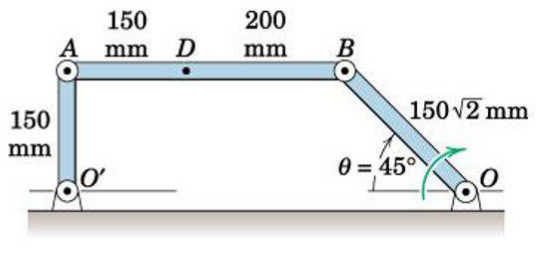
\includegraphics[height=6cm,width=0.6\textwidth,keepaspectratio]{image24.png}
        \caption*{Task 1}
        \label{fig:image24}
    \end{figure}
\end{frame}

\begin{frame}[t]{Task 1 (yours): solution}
\framesubtitle{}
    \begin{figure}[H]
        \centering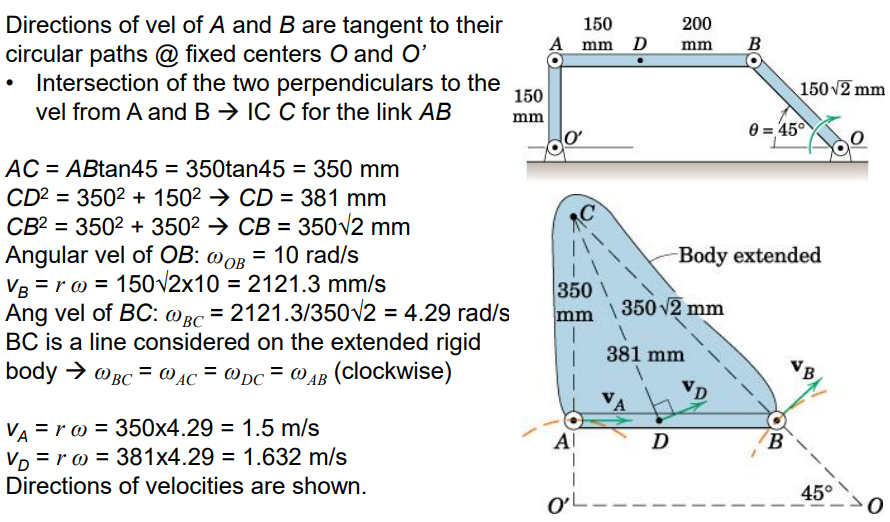
\includegraphics[height=6cm,width=1\textwidth,keepaspectratio]{image20.png}
        \label{fig:image20}
    \end{figure}
\end{frame}

\begin{frame}[t]{Task 2 (mine)}
\vspace{-0.4cm}
\begin{minipage}{0.55\textwidth}
The task to find kinematics for the whole mechanism and velocities for $D$.
\bigskip

You know all lengths $(OA, AB, BC)$, $\varphi(t)$. \\ Coordinates of all bases are known. The basis near to $M$ point is horizontal respect to the ground.
\end{minipage}
\begin{minipage}{0.42\textwidth}
        \begin{figure}[H]
    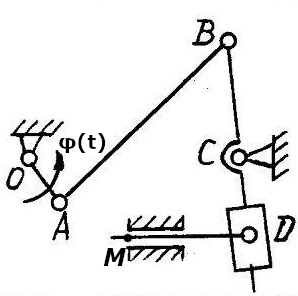
\includegraphics[width=0.9\textwidth]{lab4_task2_fig.png}\\
    \caption*{Task 2}
    \end{figure}
\end{minipage}
\end{frame}

\section*{Tasks --- Spherical motion}

\begin{frame}[t]{Task 3 (mine)}
    \begin{minipage}{0.42\textwidth}
    The cone (angle --- $2\alpha,\ \alpha = 30^\circ,\ r=20$ --- base) is rolling on a ground without friction. $\vec{V}_C=const=60$.
    \\
    It is needed to find $\Omega,\ \varepsilon,\ \vec{V}_B,\ \vec{a}_B$.
    \end{minipage}
    \begin{minipage}{0.55\textwidth}
            \begin{figure}[H]
        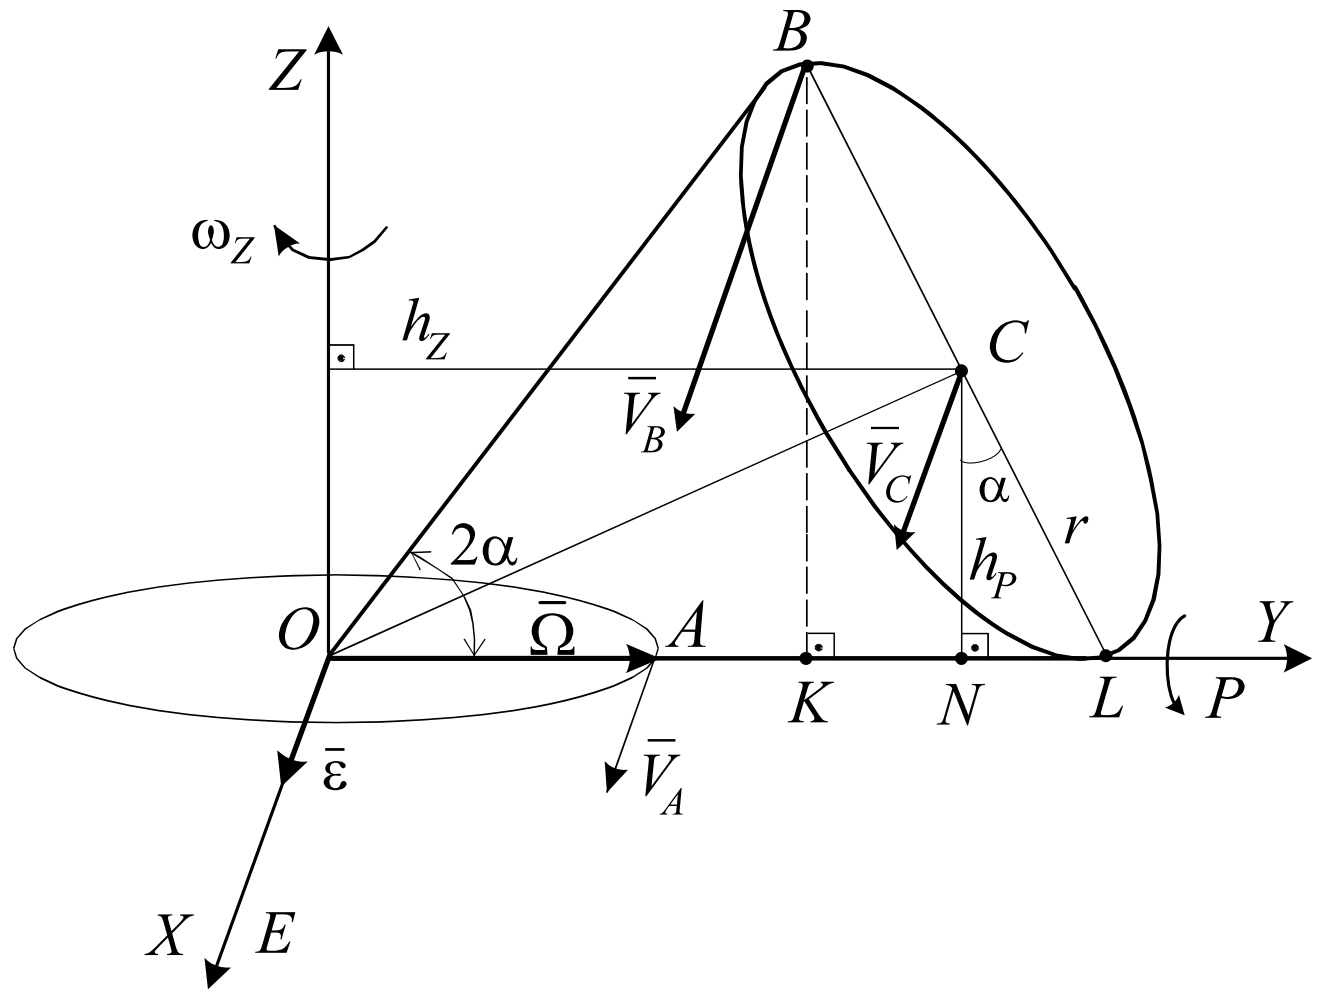
\includegraphics[width=0.9\textwidth]{lab4_task3_filled_fig.png}\\
        \caption*{Task 3}
        \end{figure}
    \end{minipage}
\end{frame}

\begin{frame}[t]{Task 3 (hints)}
\framesubtitle{}
    \begin{figure}[H]
        \begin{subfigure}{0.59\textwidth}
            \centering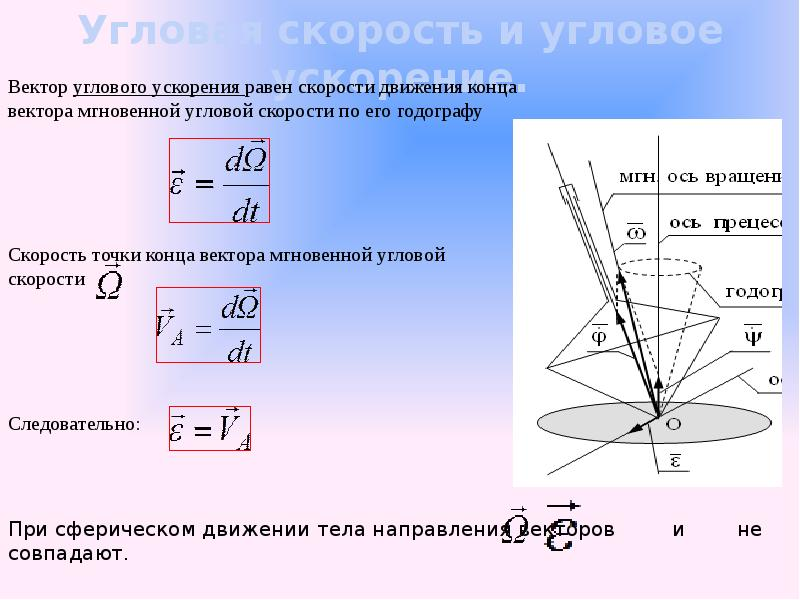
\includegraphics[height=5cm,width=1\textwidth,keepaspectratio]{image10.png}
            \label{fig:image10}
        \end{subfigure}
        \begin{subfigure}{0.4\textwidth}
            \centering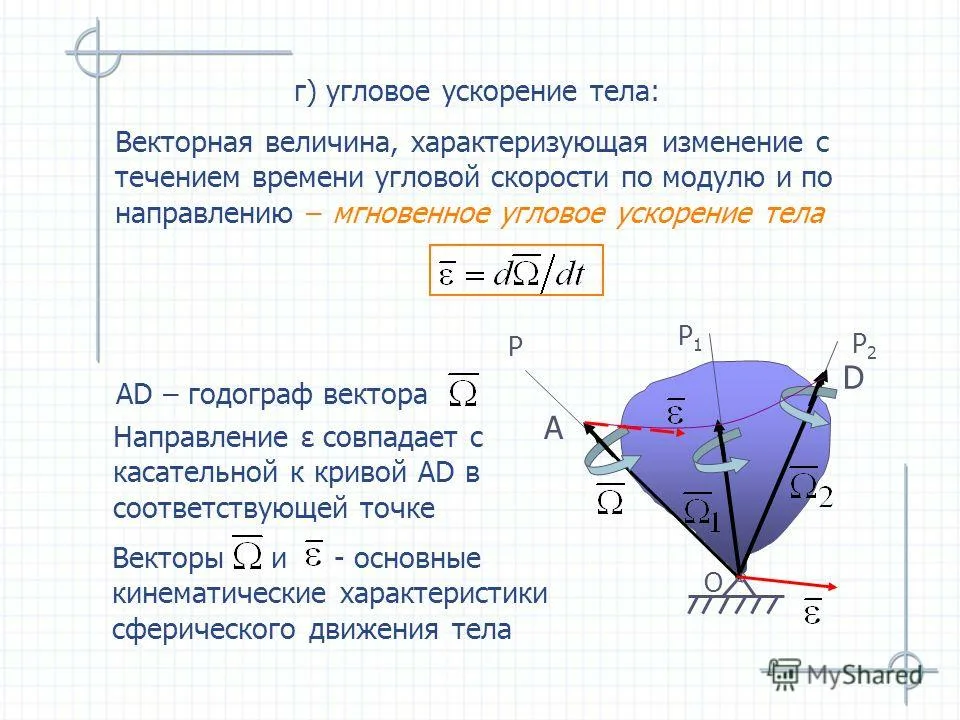
\includegraphics[height=5cm,width=1\textwidth,keepaspectratio]{image25.png}
            \label{fig:image25}
        \end{subfigure}
    
    \label{fig:}
    \end{figure}
\end{frame}

\begin{frame}[t]{Task 4 (yours): M (rus) 19.9}
\framesubtitle{}
    \begin{figure}[H]
        \begin{subfigure}{0.79\textwidth}
            \centering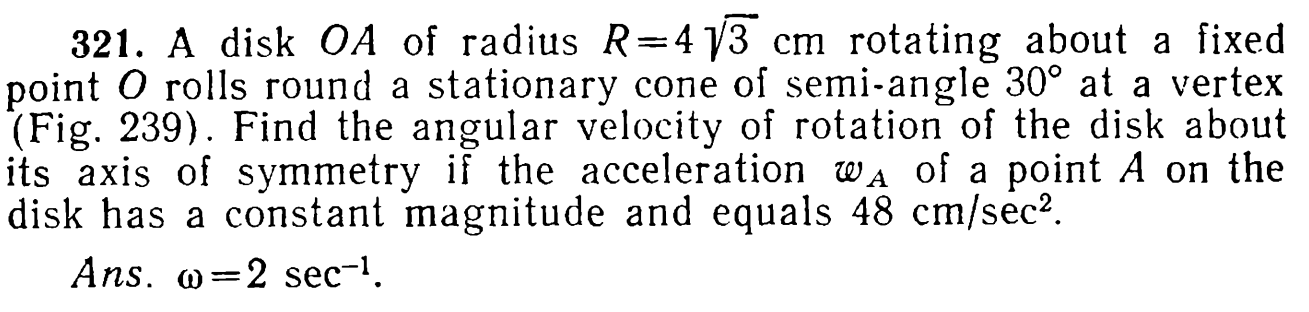
\includegraphics[height=6cm,width=1\textwidth,keepaspectratio]{image12.png}
            \label{fig:image12}
        \end{subfigure}
        \begin{subfigure}{0.19\textwidth}
            \centering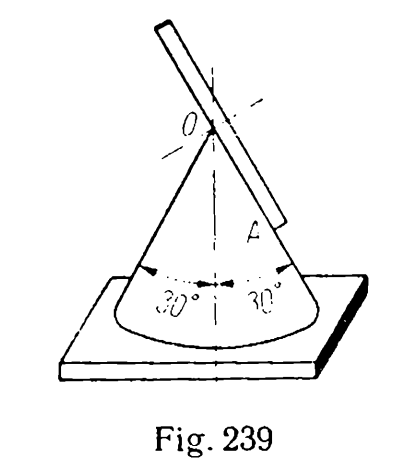
\includegraphics[height=6cm,width=1\textwidth,keepaspectratio]{image9.png}
            \label{fig:image9}
        \end{subfigure}
    \end{figure}
\end{frame}

\fbckg{fibeamer/figs/last_page.png}
\frame[plain]{}
\end{document}